\documentclass[addpoints,12pt]{exam}
%\documentclass[12pt]{article}
\usepackage[letterpaper, margin=0.75in]{geometry}
\usepackage{graphicx}
\usepackage{enumitem}
\usepackage{booktabs}
\usepackage{tabularx}
\usepackage{amsmath}
\usepackage[makeroom]{cancel}
\begin{document}
\footer{}{Page \thepage\ of \numpages}{}


\begin{center}

\includegraphics[width=10cm]{../images/logo.png}
\end{center}

\begin{center}
\noindent{\LARGE Conceptual Physics \\ Homework Packet 2\\ Solutions \\}
\end{center}
 
\clearpage

\begin{flushright}
Score: \hspace{0.2in} / \numpoints ~ points
\end{flushright}


\begin{questions}
\question[2]
Is it possible for speed to be constant while acceleration is not zero? If \textit{yes}, give an example. If \textit{no}, explain why not. (Feel free to include a diagram.)

From: \textit{College Physics,} Ch.2, Conceptual Question 13

\begin{TheSolution}
Yes, it is possible. Driving around a circle at a constant speed, yet changing direction results in constant speed with non-zero acceleration.
\end{TheSolution}

	\question[4]
	A car begins speeding up from rest, accelerating at a constant rate of $6~\text{m}/\text{s}^2$.
	\begin{parts}
		\part How long does it take to reach a velocity of 30 m/s?
			\begin{TheSolution}
			We know the car's acceleration ($6~m/s^2$), initial velocity (rest, not moving) and final velocity ($30~m/s$). We are looking for time, and so we can use the basic relation between acceleration, velocity and time:
				\begin{eqnarray}
				a &=& \frac{\Delta v}{\Delta t} \nonumber\\
				 &=& \frac{v_f - v_i}{t} \nonumber
				\end{eqnarray}
				Using the numbers, we have:
				\begin{eqnarray}
				6~m/s^2 &=& \frac{30~m/s - 0}{t} = \frac{30~m/s}{t}\nonumber \\
				t &=& \frac{30~m/s}{6~m/s^2} = 5~s\nonumber
				\end{eqnarray}
			\end{TheSolution}
		\part How far does it travel in this time?
			\begin{TheSolution}
				We can use the kinematic equations that relate time, velocity and acceleration:
				\begin{eqnarray}
				x = v t +\frac{1}{2}at^2\nonumber
				\end{eqnarray}
				We know the acceleration ($6~m/s^2$), initial velocity ($0~m/s$) and time ($5~s$) and so we can find the distance:
				\begin{eqnarray}
				x &=& 0~m/s\times 5s + \frac{1}{2}(6~m/s^2)\times(5~s)^2\nonumber \\
				&=& \frac{6\times 5^2}{2} m \nonumber\\
				&=& \frac{6\times 25}{2}m = 3\times 25~m = 75~m\nonumber
				\end{eqnarray}
			\end{TheSolution}
	\end{parts}
	
	\question[4]
The North American and European continents, which are about 6000 km apart, are moving apart at a rate of about 2~cm/year.

\begin{parts}
\part Assuming this rate has remained constant since they began separating, when did they start separating?
\begin{TheSolution}
Here we all looking for time, when we have distance and a speed. 
\begin{eqnarray}
speed &=& \frac{distance}{time} \nonumber\\
2~cm/year &=& \frac{6000~km}{t} \nonumber
\end{eqnarray}
Here we have different units, so we need to make sure we convert to the same units in order to compare. Since we cm and km, it would be easiest to convert both to meters:
\begin{eqnarray}
\frac{2~\cancel{cm}}{year}\times\frac{1~m}{100~\cancel{cm}} &=& \frac{6000~\cancel{km}}{t}\times\frac{1000~m}{\cancel{km}} \nonumber \\
\frac{2~m}{100~year} &=& \frac{6,000,000~m}{t} \nonumber \\
\frac{1~m}{50~year} &=& \frac{6,000,000~m}{t} \nonumber
\end{eqnarray}
We rearrange the fractions to find \textit{t}:
\begin{eqnarray}
t &=& \frac{6,000,000~m}{1~m}\times\frac{50~years}{1} \nonumber \\
&=& 300,000,000~years = (3.0\times 10^8 years)\nonumber \\
&=& 300~million~years \nonumber
\end{eqnarray}
\end{TheSolution}

\part If new evidence was uncovered that the plates were steadily slowing down, how would this affect your answer (\textit{i.e.}, would it have taken more or less time for the plates to separate to their current distance)?
\begin{TheSolution}
We would need to take into consideration that the speed was changing. If the plates are slowing down, then in the past they were moving faster. It would therefore take \textit{less time} to cover the same distance.
\end{TheSolution}
\end{parts}


	\question[3]
	You are looking into a deep well. It is dark, and you cannot see the bottom. You want to find out how deep it is, so you drop a rock in, and you hear a splash 3.0 s later. How deep is the well? (For simplicity, let the acceleration due to gravity be $g=10~m/s^2$)
	
	From: \textit{Light and Matter,} Ch. 3, Question 9
	\begin{TheSolution}
		We know the initial velocity (zero, since at rest), the acceleration ($10~m/s^2$) and the time (3.0~s). We are looking for distance, and so we can use the following kinematic equation:
		\begin{eqnarray}
		x &=& vt+\frac{1}{2}at^2 \nonumber \\
		&=& 0~m/s\times (3~s) + \frac{1}{2}(10~m/s^2)\times(3~s)^2\nonumber\\
		&=& \frac{10\times 3^2}{2}m\nonumber\\
		&=& 5\times 9~m = 45~m \nonumber
		\end{eqnarray}
	\end{TheSolution}

\question[4]
Your friend makes the following graphs of the \textbf{position} and \textbf{velocity} of an object as a function of time, but forgets to label the axes. He tells you the object was undergoing constant acceleration. Which plot is which? \textbf{Label the axes}. (Be sure to label both horizontal axis, as well as both vertical axis).
\begin{TheSolution}
In both cases, we know that the horizontal axis is time. Also, we know that acceleration is constant, and so the velocity versus time graph must be straight (not curved). Therefore, (a) must be the velocity versus time graph. By elimination, (b) is the position versus time graph.

\noindent
     \begin{tabularx}{0.8\textwidth}{ X X }
     
     (a) \raisebox{-\totalheight}{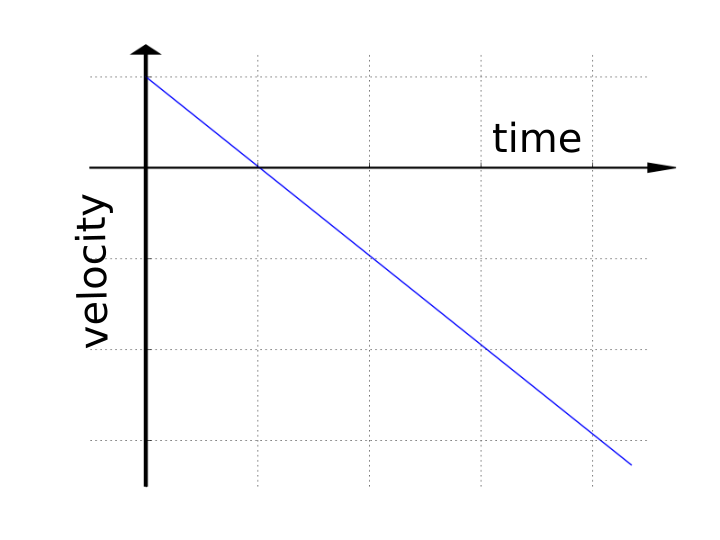
\includegraphics[width=0.45\textwidth]{../images/hw3_v_sol.png}}
      & 
      (b) \raisebox{-\totalheight}{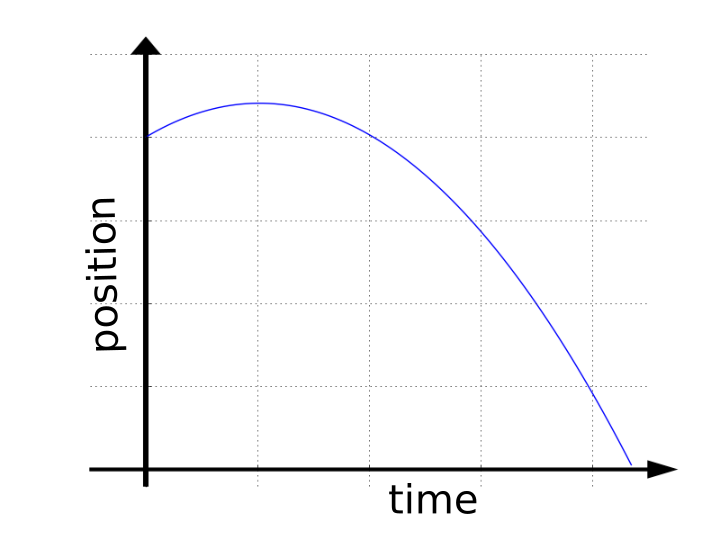
\includegraphics[width=0.45\textwidth]{../images/hw3_x_sol.png}}\\
      \end{tabularx}
\end{TheSolution}

	
\clearpage
	 \question[8]
You walk down a 10 m hallway at a constant speed in 10 s, pause for 5 s, then turn around and jog back to your initial position in another 5 s (again at a constant speed).
\begin{parts}
	\part Using the grid below, plot position as a function of time. Assume you begin walking at t=0 s.
	\begin{center}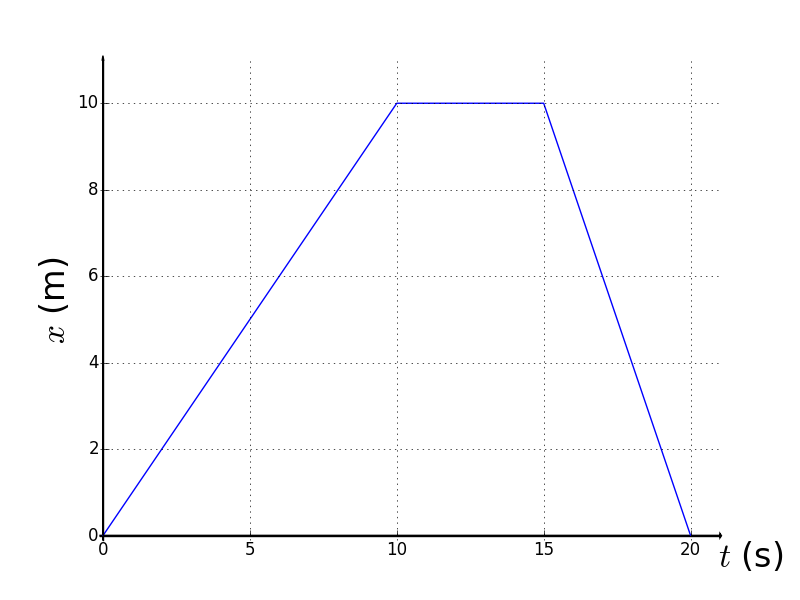
\includegraphics[width=0.75\textwidth]{../images/hw3_hallwaysol.png}\end{center}
	\part Using the grid below, plot velocity as a function of time. Assume you begin walking at t=0 s.
	\begin{center}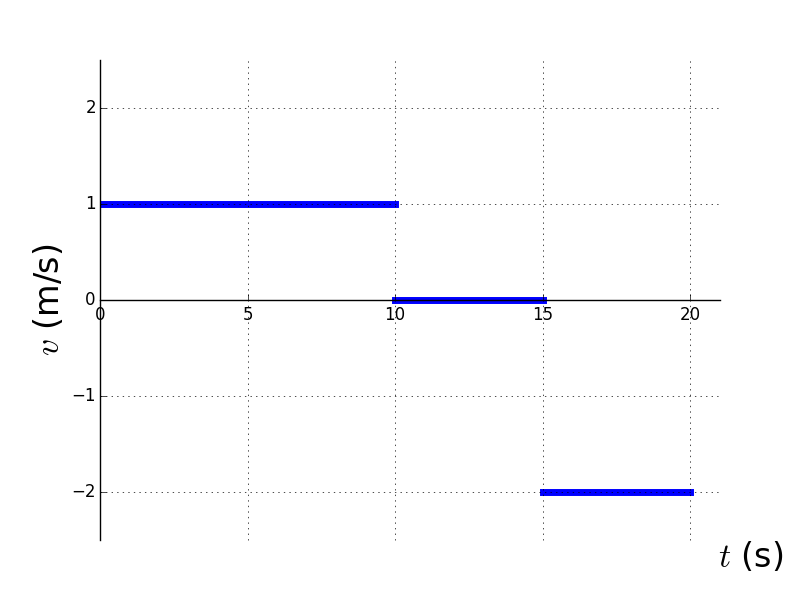
\includegraphics[width=0.75\textwidth]{../images/hw3_hallwayvsol.png}\end{center}
	\part What is the distance traveled?
		\begin{TheSolution}
			You travel 10~m down and 10~m back: total of 20~m.
		\end{TheSolution}
	\part What is you average speed?
		\begin{TheSolution}
			Speed is found by looking at distance divided by time.
			\begin{eqnarray}
				speed = \frac{distance}{time} = \frac{20~m}{20~s} = 1~m/s. \nonumber
			\end{eqnarray}
		\end{TheSolution}
	\part What is your displacement?
		\begin{TheSolution}
			Since you began and ended at the same spot, the total displacement is zero.
		\end{TheSolution}
	\part What is your average velocity?
		\begin{TheSolution}
			Velocity is found by looking at displacement divided by time. Since the displacement is zero (and the time is 15~s, not zero) the velocity is zero.
		\end{TheSolution}
	\part What is your instantaneous velocity at t=5~s?
		\begin{TheSolution}
			The slope at that point is found by looking at::
			\begin{eqnarray}
			\frac{10~m}{10~s} = 1~m/s \nonumber
			\end{eqnarray}
		\end{TheSolution}
	\part What is your instantaneous velocity at t=18~s?
		\begin{TheSolution}
		At this point you are walking back, so it is negative. We can therefore find it by looking at:
		\begin{eqnarray}
		\frac{-10~m}{5~s} = -2~m/s \nonumber
		\end{eqnarray}
		\end{TheSolution}
\end{parts}
	 
	 \bonusquestion[2]
Our Solar System is orbiting the center of the Milky Way Galaxy, which is about 28,000 light-years ($2.7\times 10^{17}$~km) away, in a roughly circular orbit.	 One orbit is called a galactic year and it takes about 250 million Earth years to complete.
\begin{parts}
\part What is the Solar System's average speed around the center of the galaxy? The answer can be in whatever units you're more comfortable with (km/s, miles/hour, km/year, etc.). A useful constant is $\pi = 3.14159... = 3$ (rounded for convenience).
	 \begin{TheSolution}
	 	The average speed is found by looking at the distance divided by total time. The total distance is the circumference of the circle traveled by the Earth:
	 	\begin{eqnarray}
	 	c &=& 2\pi r = 2\times 3\times 2.7\times 10^{17} km \nonumber \\
	 	&=& 16.2\times 10^{17} km = 1.62\times 10^{18}~km \nonumber
	 	\end{eqnarray}
	 	Using this, we can find the speed by looking at the distance over time:
	 	\begin{eqnarray}
	 	speed &=& \frac{1.62\times 10^{18}~km}{250~million~years} = \frac{1.62\times 10^{18}~km}{250\times 10^6~years} = \frac{1.62\times 10^{18}km}{2.5\times 10^8~years} \nonumber \\
	 	&=& 0.65\times 10^{10}~km/years = 6.5\times 10^{9}~km/year
	 	\end{eqnarray}
	 \end{TheSolution}
\end{parts}
	 
	 \begin{center}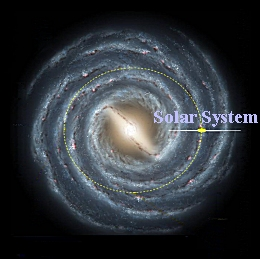
\includegraphics[width=0.4\linewidth]{../images/MilkyWaySolarSystem.jpg}\end{center}
	 
\end{questions}








\end{document}